%%
%  ******************************************************************************
%  * #file    Szablon_raportu_EN_Latex.tex
%  * #author  Adrian Wójcik   adrian.wojcik(at)put.poznan.pl
%  *          
%  * #commit  Patryk Kościk   koscikpatryk(at)gmail.com
%  *          Modified the template for Projekt przejsciowy purposes          
%  *          
%  * #version 1.0
%  * #date    09-Mar-2022
%  * #brief   PROJPRZEJ
%  *
%  ******************************************************************************
%%  
\documentclass[11pt, a4paper]{article}

\usepackage{SM_template}

% Wypełnijcie te dyrektywy zgodnie z waszym tematem
% \lab      -> NAZWA CZUJNIKA, np.: 'DHT22'
% \comment  -> Króciutki opis co to, np.: 'Cyfrowy budżetowy czujnik temperatury'
%
\lab{KNY-015: DHT-11}
\comment{Cyfrowy czujnik wilgotności i temperatury otoczenia \\ Szymon Kwiatkowski}

% Absolutny zakaz dotykania tego tutaj bo jak dotkiecie to coś jebnie
\university{Politechnika Poznańska}
\faculty{Wydział Automatyki, Robotyki i Elektrotechniki}
\institute{Instytut Robotyki i Inteligencji Maszynowej}
\department{Zakład Sterowania i Elektroniki Przemysłowej}
\addbibresource{bib/DHT_11.bib}
\nocite{*}


%%
%
% Początek dokumentu
%
%%
\begin{document}

%% Strona tytułowa %%
\mainpage{{DHT11/DHT_11.jpg}}
\newpage

\section*{Opis elementu} \addcontentsline{toc}{section}{Wstęp}
Czujnik przez nas rozpatrywany jest czujnikiem cyfrowym i posiada 2 wejścia oraz jedno wyjście które nas interesuje podczas transmisji danych:
\begin{itemize}
    \item VCC - wejście zasilające(5V)
    \item GND - masa układu
    \item DOUT - wyjście cyfrowe danych układu
\end{itemize}
Wyjście DOUT jest w praktyce pinem GPIO, który jest odpowiednio przystosowany do czytania informacji na nim się pojawiających.

Sam moduł wygląda również następująco w praktyce:
\begin{figure}[H]
    \centering
    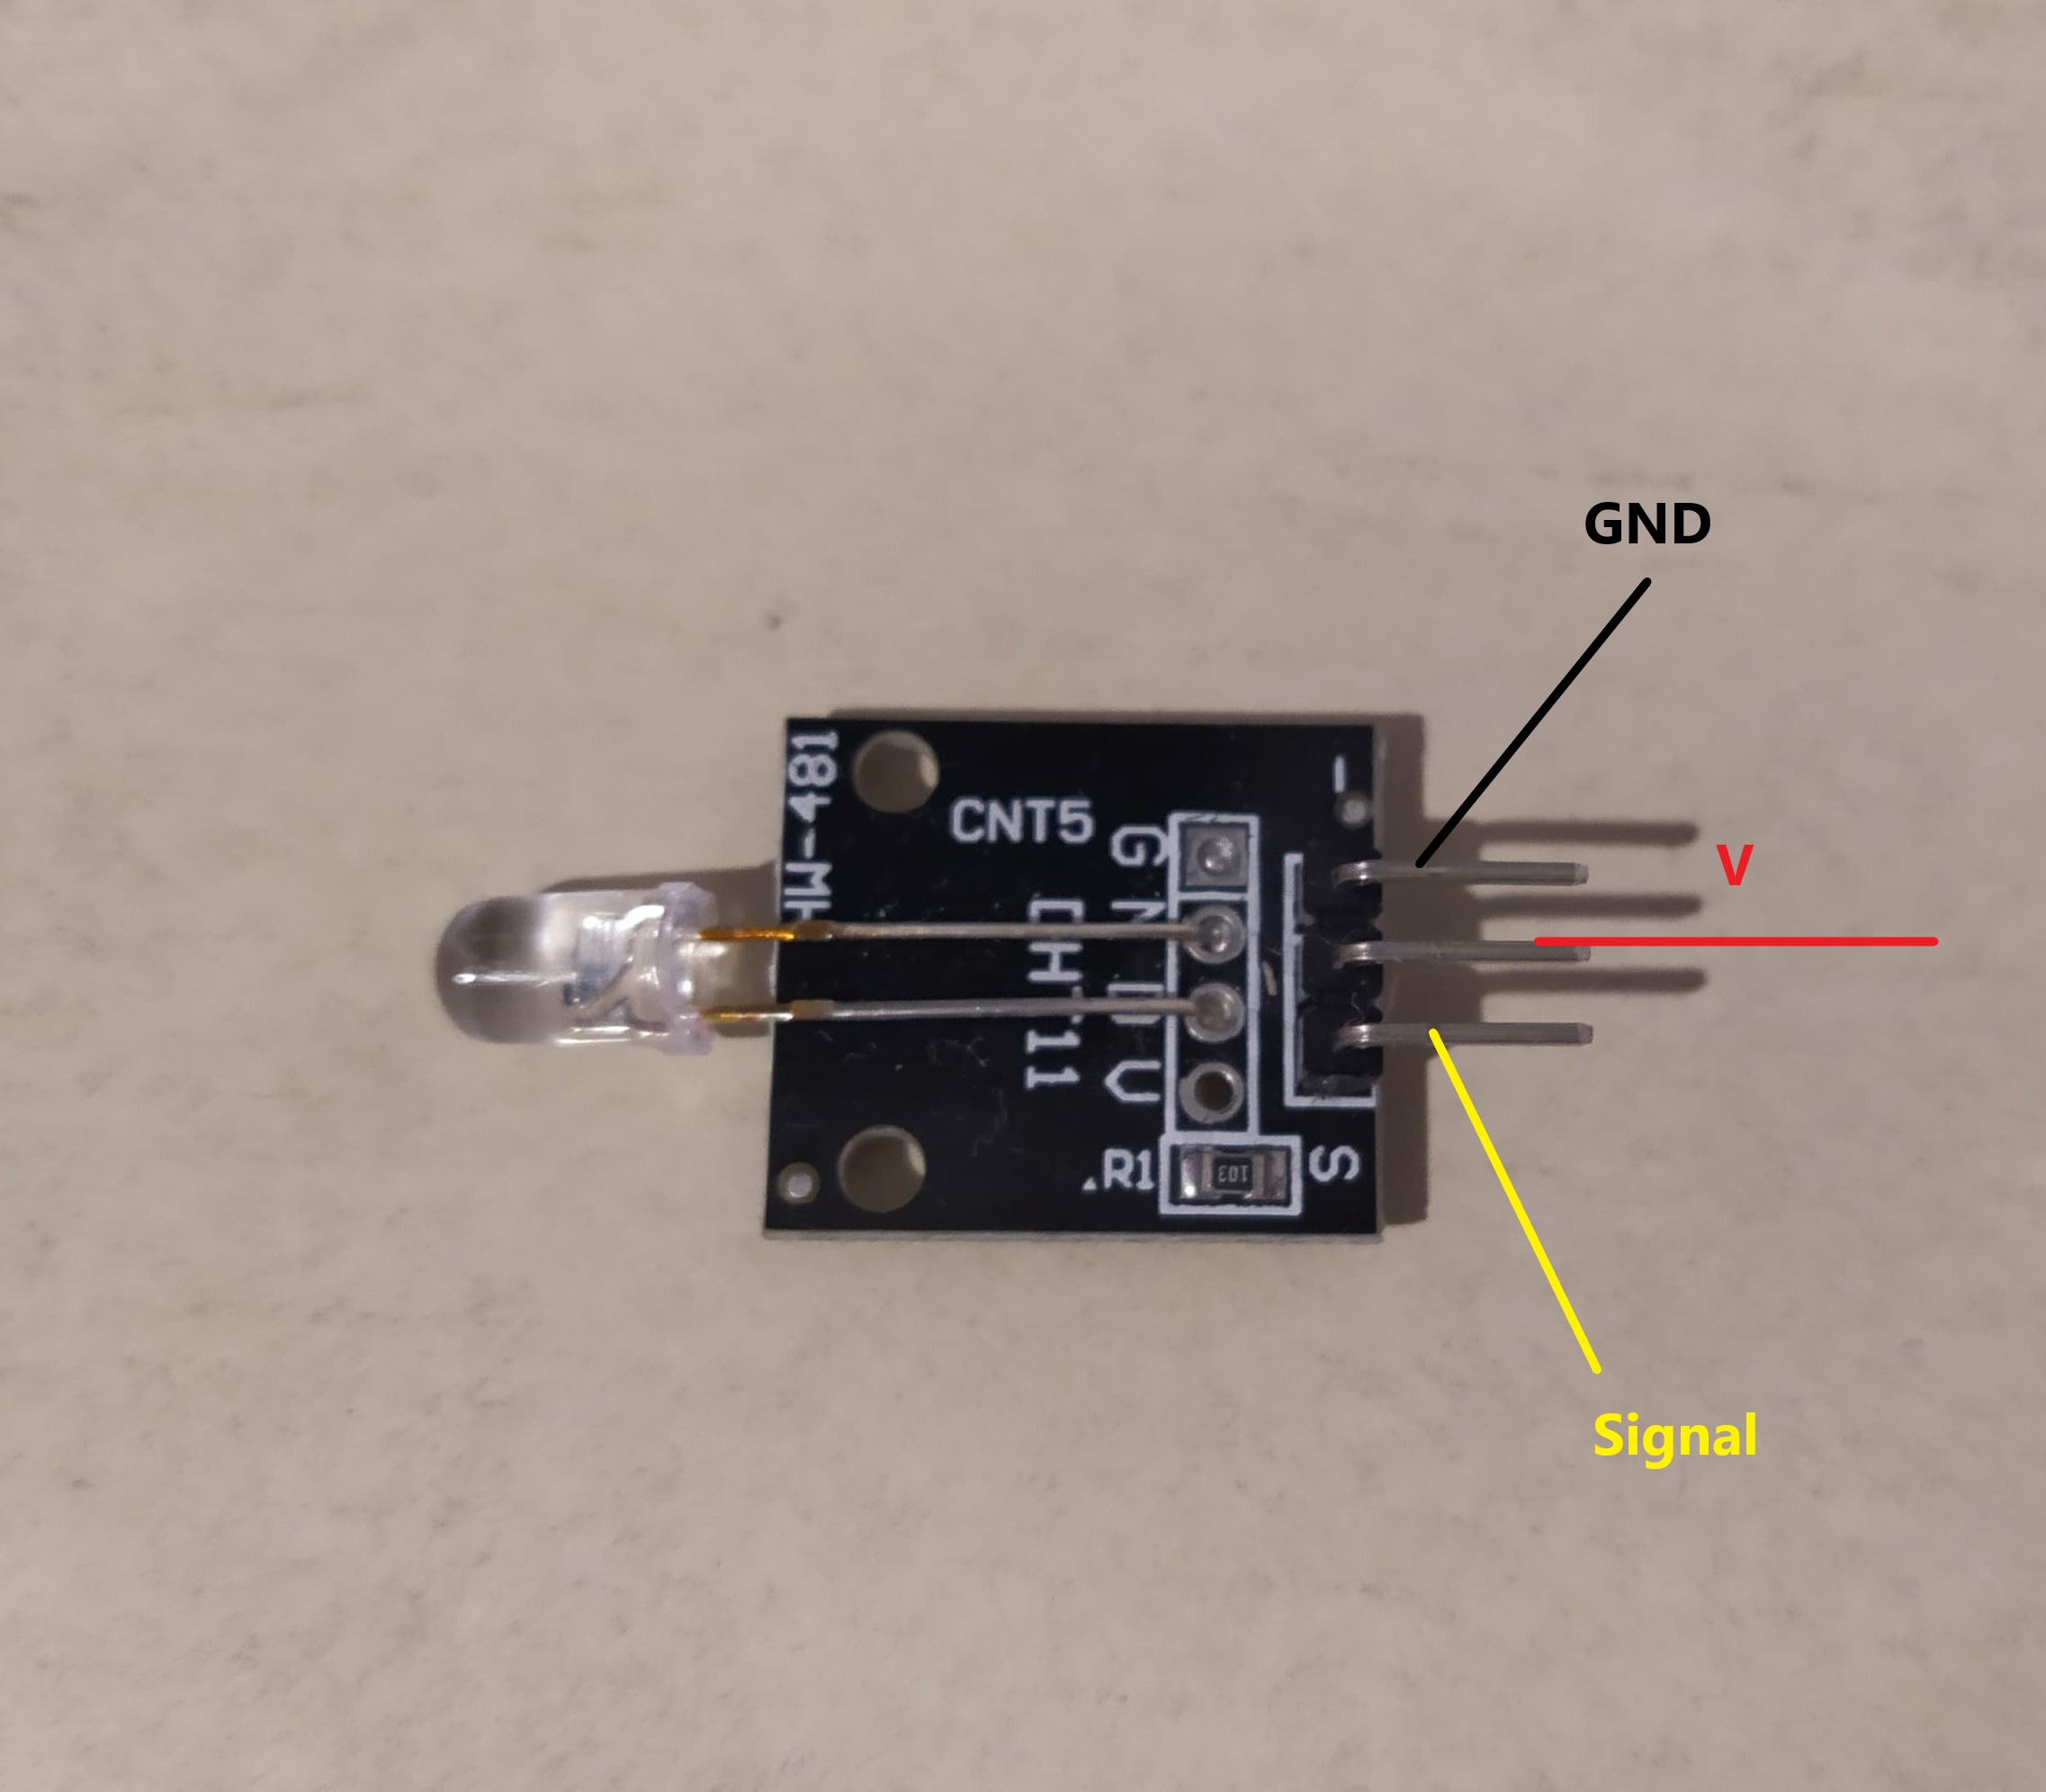
\includegraphics[width=0.4\textwidth]{fig/DHT11/zdj_modułu/fig1.jpg}
    \caption{Piny modułu}
    \label{fig:fig1}
\end{figure}

Czujnik jest cyfrowy i wysyła nam informacje które są kodowane na kilku bajtach. Dwa pierwsze bajty informacji to aktualna temperatura, następne dwa to aktualna wilgotność i na sam koniec otrzymujemy 1 bajt który pełni funkcje parity. Użycie ostatniego bajtu pozwala zweryfikować czy otrzymane przez nas infromacje są odpowiednio otrzymane i tym samym w prosty sposób je zwalidować. Aby móc stwierdzić czy wiadomości dotarły poprawnie należy po prostu zsumować kolejne bajty otrzymanych przez nas wiadomości co ostatecznie pozwoli na zweryfikowanie otrzymanej wartości poprzez proste przyrównanie do parity bajtu. To że posiadamy dokładnie 5 bajtów oznacza że otrzymujemy łącznie 40 informacji. Informacje te są kodowane w specyficzny sposób z którym należy zapoznać się w dokumentacji przed rozpoczęciem pracy z czujnikiem. Kodowanie bowiem odbywa się za pomocą czasu trwania stanu wysokiego podczas wysyłania wiadomości. Jeżeli stan wysoki w odpowiedzi na sygnał hosta trwa około 24 do 26 mikrosekund to otrzymujemy tam wartość binarną równą 0. Jeżeli odpowiedź trwa około 70 mikrosekund to jest to równoznaczne z otrzymaniem wartości binarnej równej 1. Dobrze ilustruje to przedstawione w dokumentacji wykresy.
\begin{figure}[H]
    \centering
    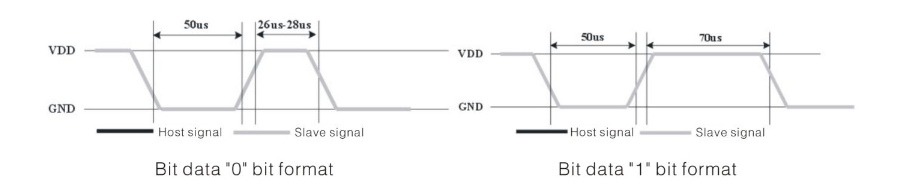
\includegraphics[width=0.8\textwidth]{fig/DHT11/zasada_dzialania/Transmisjadanych.png}
    \caption{Przebieg transmisji danych modułu po szeregowym wyjściu DOUT}
    \label{fig:fig1}
\end{figure}
Wnioskując zatem po powyższej grafice możemy zauważyć że pin GPIO do które podłączymy nasz mikrokontroler będzie musiał pracować zarówno jako wyjście(kiedy zmieniamy sami stan pojawiający się na wyjściu przez 50 mikrosekund), jak i jako wejście(kiedy skończymy pracować jako wyjście i chcemy zebrać informacje które zaraz pojawią się na DOUT).


\newpage

\section{Użycie czujnika}
Jak już wcześniej zauważono posiadamy zaledwie 3 piny naszego modułu z czego dwa pracują jako wejścia, a jeden jako wejście. Można zatem zauważyć że samo podłączenie nie jest skomplikowane. Jednak sam moduł DHT-11 w podłączeniu różni się minialnie od naszego gotowego modułu i wymaga kilku zmian praktycznych.
\begin{figure}[h!]
    \centering
    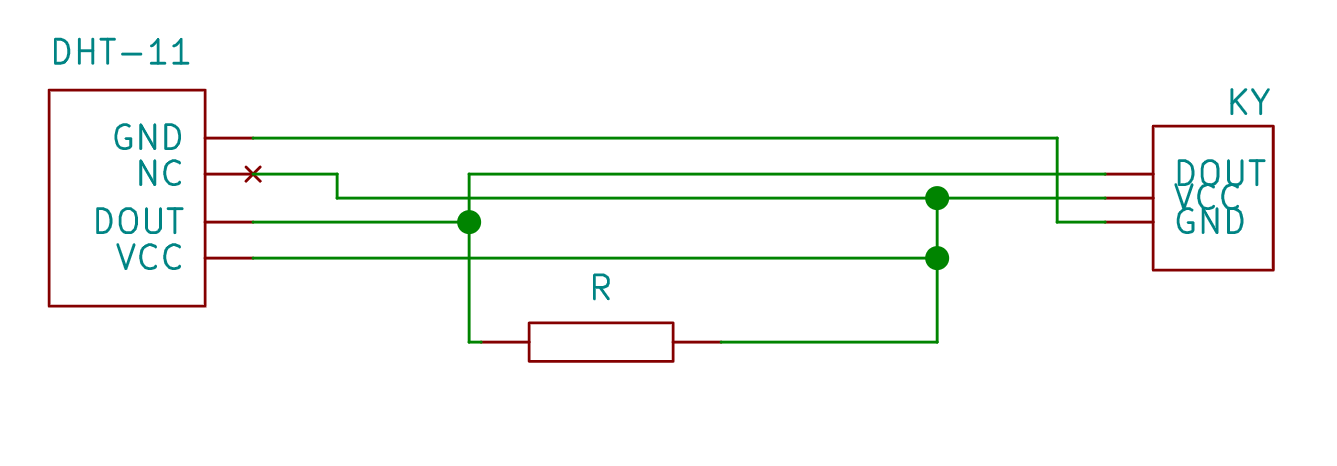
\includegraphics[width=0.6\textwidth]{fig/DHT11/polaczenie_modulu/schematPodlaczenia.png}
    \caption{Połaczenie elektryczne modułu}
    \label{fig:my_label}
\end{figure}
Jak można zatem zauważyć posiadamy nadal równie dużo sygnałów jednak samo sposób ich podłączenia pod DHT-11 lekko się różni. Pierwszą ważną rzeczą którą trzeba zauważyć jest to że linia DOUT jest poprowadzona poprzez rezystor pullup. Dodatkowo pojawia sie jedno więcej wejście NC, które w prosty sposób można przetłumaczyć jako not connected. W przypadku naszego modułu mimo mylącej nazwy jest podłączone jednak nie jest konieczne to aby tak jak w naszym przypadku było ono koniecznie podłączone do 5V.


Korzystając z samego czujnika i posiadając wiedzę na jego temat jesteśmy w stanie z niego korzystać. Nie można odczytywać z niego informacji za pomocą magistrali szeregowej, jednak wystarczy odpowiednio przygotować projekt tak aby umożlwiał nam:
\begin{enumerate}
    \item Odliczanie opóźnień czasowych w milisekundach
    \item Zmieniał tryb operowania pinu tak aby mógł pracować zarówno jako wejście i wyjście w zależności od naszych zapotrzebowań
    \item Zrealizować logiczny sposób czytania danych pojawiających się na linii DOUT
\end{enumerate}
Ważną uwagą odnośnie pracy z układem jest to aby konfigurując pin z którego będziemy mieli korzystać do odczytu danych ustawić jego pole: \newline
\textbf{GPIO output level: High}


Układ po podłączeniu do samego zasilania prezentował się następująco: 
\begin{figure}[h!]
    \centering
    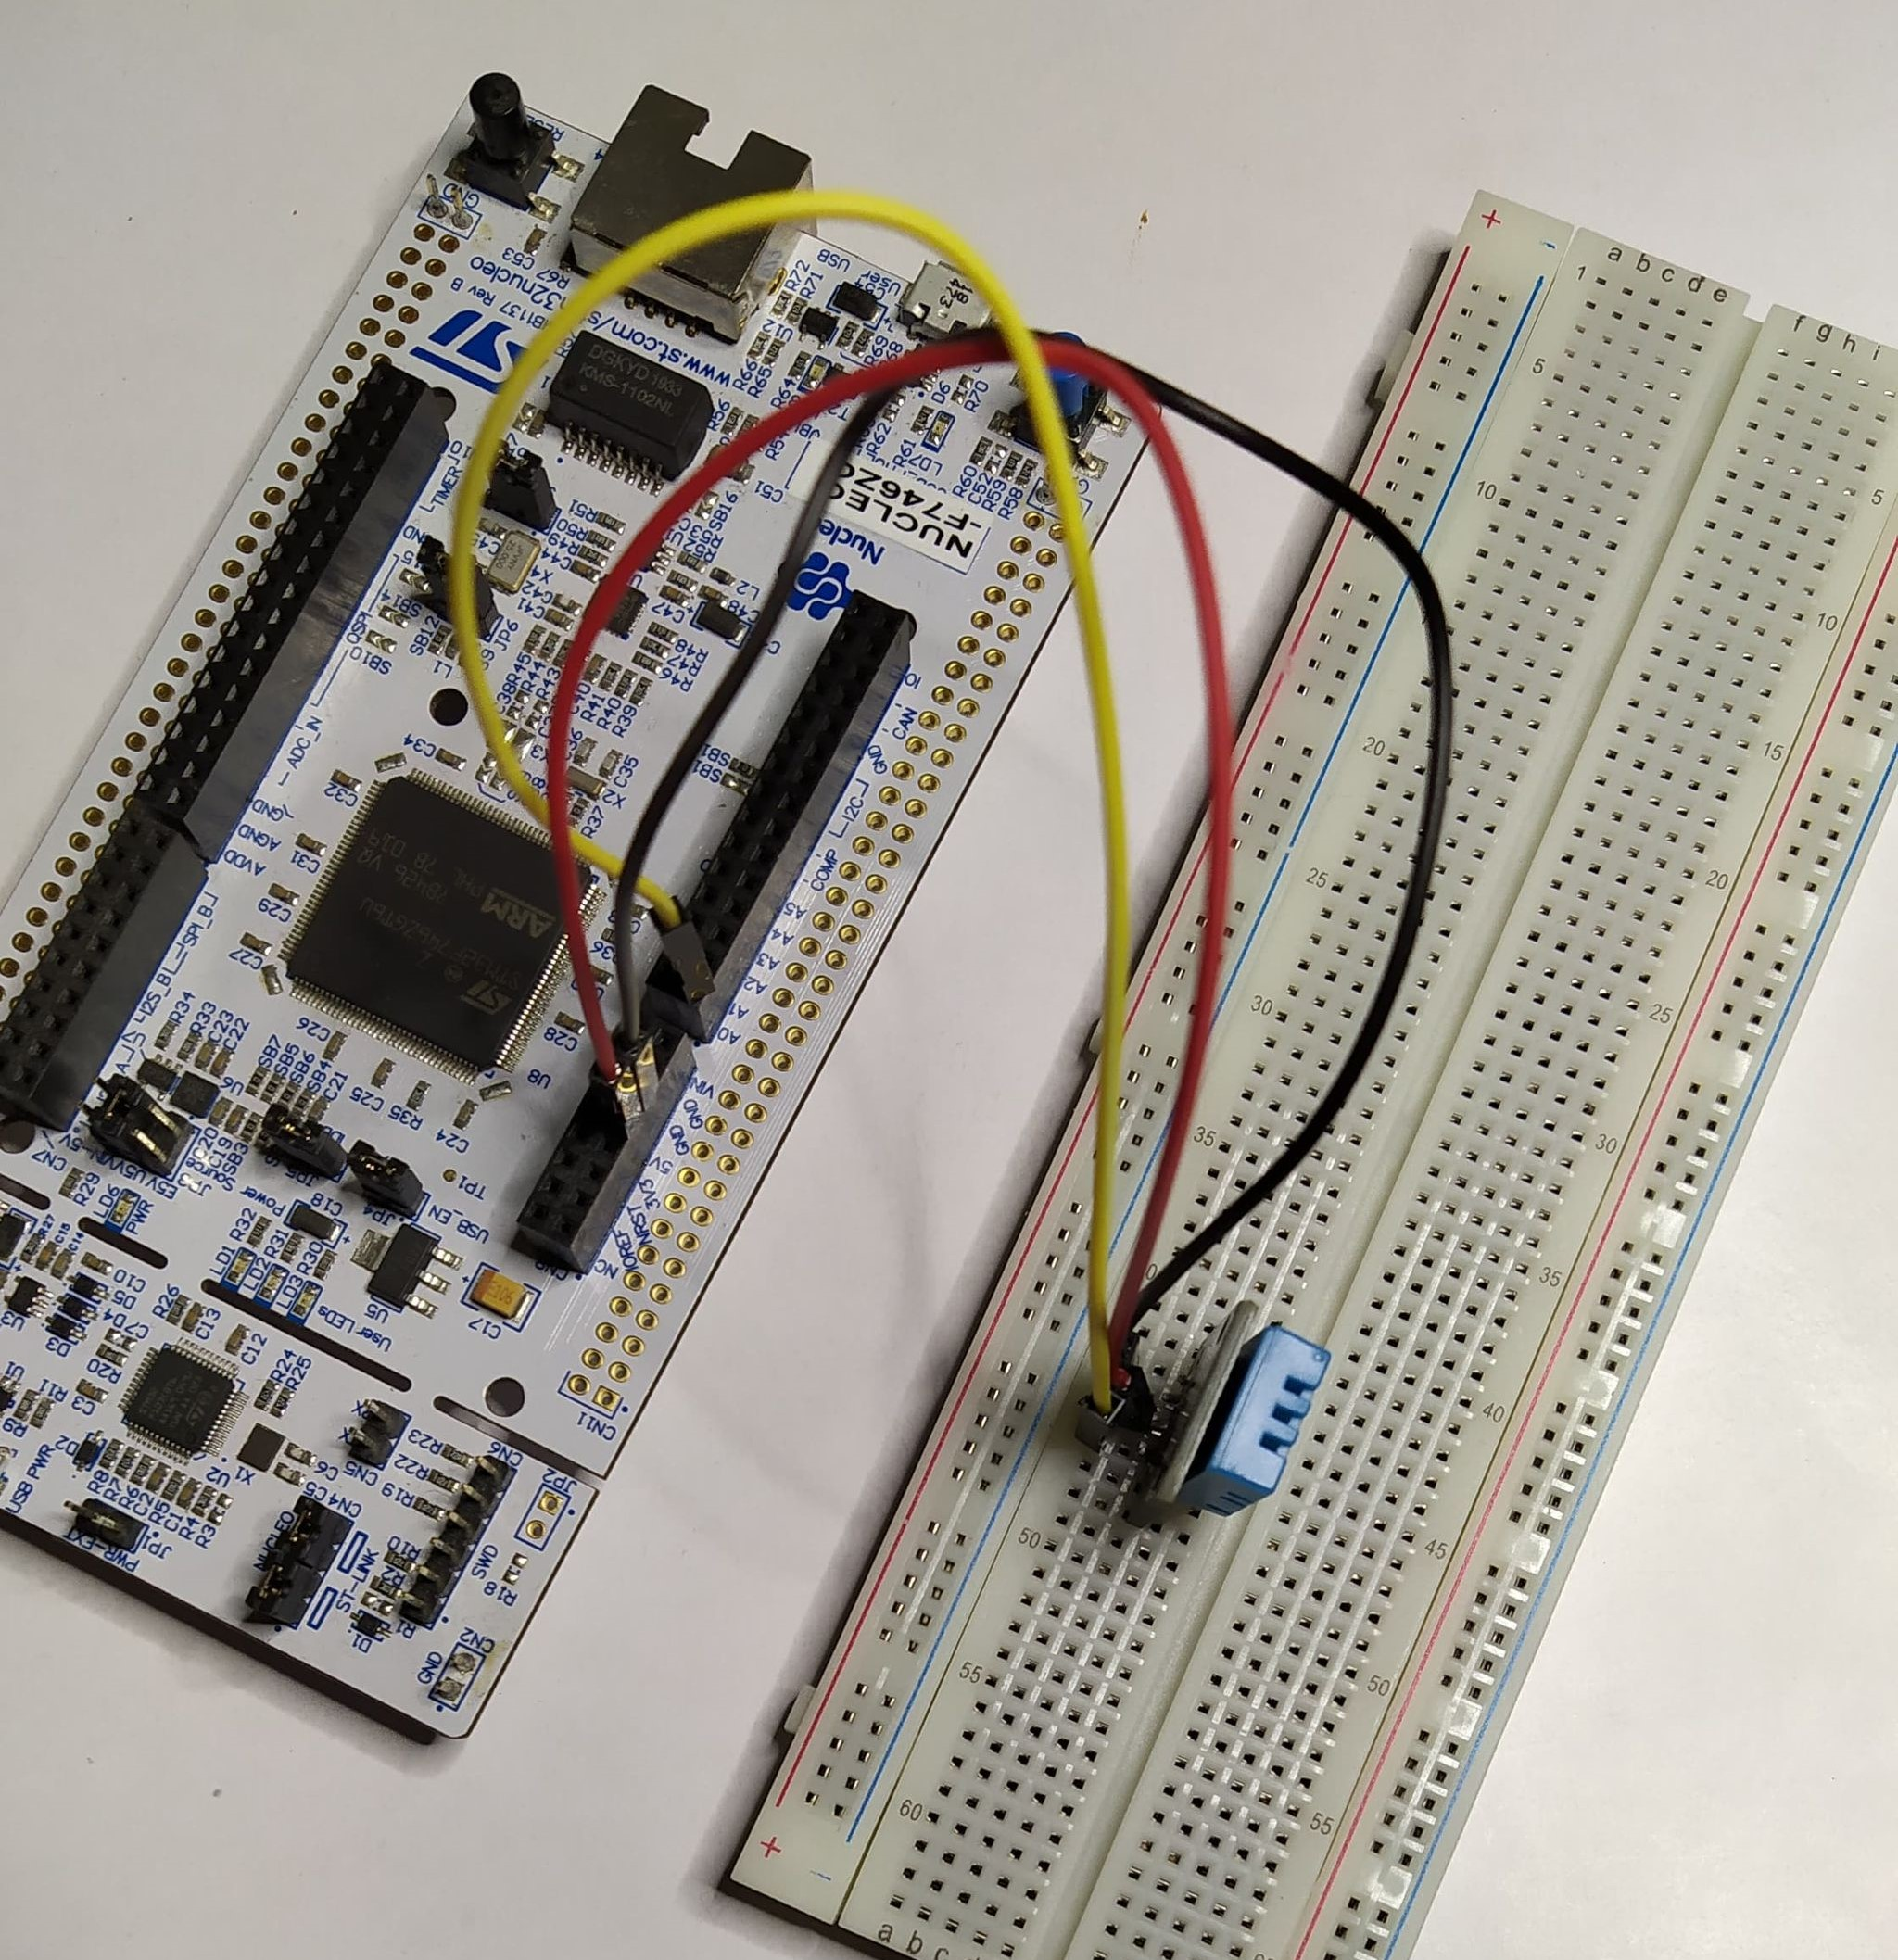
\includegraphics[width=0.4\textwidth]{fig/DHT11/działanie_ukladu/Podlacznie.jpg}
    \caption{Realizacja praktyczna układu}
    \label{fig:dzialanie}
\end{figure}

\newpage
\printbibliography[heading=bibintoc]

\end{document}